%%%%%%%%%%%%%%%%%%%%%%%%%%%% Document Class %%%%%%%%%%%%%%%%%%%%%%%%%%%% 
\documentclass{report} % use larger type; default would be 10pt

%%%%%%%%%%%%%%%%%%%%%%%%%%%% PACKAGES TO USE %%%%%%%%%%%%%%%%%%%%%%%%%%%%
%%%%% Page Style %%%%%
\usepackage[margin=1.0in]{geometry}            	% setting the side margins to be ______ inches
\usepackage{fancyhdr}                             		% used to better a custom footer with names/classes/total pages/...
\usepackage{lastpage}                                    	% used to calculate the total page number
%%%%% Functionality %%%%%
\usepackage{enumerate}                                	% making lists       
\usepackage{amsmath}                                   	% includes some math equation functions
\usepackage{graphicx }                                   	% including figures
%\usepackage{sidecap}                                      	% side captions on figures instead of below captions
%%%%% Formatting %%%%%
\usepackage[labelfont=bf]{caption}                  	% setting caption labels to be bold (Table ##, Figure ##)
\usepackage{longtable}					% allows tables that are longer than a single page
\usepackage[font={small,it}]{caption}			% sets captions font to be small italics
\setlength{\belowcaptionskip}{-10pt}                	% removes the extra spacing after captions
\usepackage{color}                                    		% allows one to specify the color of a set of font
\usepackage[section]{placeins}           		% Only allows figures/tables/equations after they are called in line with text
%%%%% Bibliography %%%%% 
\usepackage{cite}                                            	% including the citation package	
\usepackage{natbib}                                        	% used in combination with \setlength to remove the extra spacing in the bibliography
\setlength{\bibsep}{0.0pt}                                	% used in combination with natbib to remove the extra spacing in the bibliography

%%%%%%%%%%%%%%%%%%%%%%%%%%%% Document Title %%%%%%%%%%%%%%%%%%%%%%%%%%%%
\title{Water Vapor Dial Users Guide}
\author{Brad Schoenrock & Robert Stillwell}    

%%%%%%%%%%%%%%%%%%%%%%%%%%% Setting the Footer %%%%%%%%%%%%%%%%%%%%%%%%%%%%
\pagestyle{fancy}
\renewcommand{\headrulewidth}{0pt}\lhead{} \chead{} \rhead{}
\lfoot{\sc Schoenrock/Stillwell} \cfoot{\normalsize \thepage\ of \pageref{LastPage}} \rfoot{\sc WV DIAL Labview}
%%%%%%%%%%%%%%%%%%%%%%%%%%% Begin Title Page %%%%%%%%%%%%%%%%%%%%%%%%%%%%
\begin{document}                    
\begin{center}
{\sc \LARGE Water Vapor Dial Labview Software} \\
\vspace{0.25in}
{\sc \Large Brad Schoenrock\\}
{\sc \Large Robert Stillwell\\}
\vspace{0.5in}
{\large NCAR
\\ \today}
\end{center}
\vspace{0.5in}
\thispagestyle{empty}

%%%%%%%%%%%%%%%%%%%%%%%%%%% Begin Content Page %%%%%%%%%%%%%%%%%%%%%%%%%%%
\newpage                               	% Making a page break to start the table of contents
\tableofcontents                     	% Making a table of contents
\thispagestyle{empty}		% Removing page number from page
\newpage      				% Making a page break to start of a document
\setcounter{page}{1}            	% Starting page counting here

%%%%%%%%%%%%%%%%%%%%%%%%%%%%%%%%%%%%%%%%%%%%%%%%%%%%%%%%%%%%%%%%%



\chapter{Acronyms and Nomenclature}
\label{CH-Acronyms}

\begin{itemize}
\item{WV DIAL: Water Vapor Differential Absorption Lidar}
\item{MCS: Multi-Channel Scaler}
\item{UPS: Universal Power Supply}
\item{HSRL: High Spectral Resolution Lidar}
\item{DB HSRL: Diode Based High Spectral Resolution Lidar}
\item{T DIAL: Temperature Differential Absorption Lidar}
\item{MFF computer: Micro Form Factor computer}
\end{itemize}
\newpage    



\chapter{Codebase}
\label{CH-Codebase}

We have used github for our version control. The github repo is located here - 

https://github.com/NCAR/WVD-MCSupdate

\noindent Instructions for how to install it as well as other software for the operations of the DIAL units is located in google drive here - 

https://docs.google.com/document/d/1IzeoFDJbz2wUmzOSmWAWuVJSXAY20Qs0wkWSpMHNQFk/edit

\noindent The software should be on each of the DIAL units already, and if those instructions were followed a shortcut to the codebase should be located on the desktop named WVD-MCSupdate. The WVD-MCSupdate directory has 4 sub directores. They are WVDoldSoftware, WVDNewArchitectureUpdate, WVDMCSupdate, and tempShare. WVDoldSoftware has a copy of the old control software. WVDNewArchitectureUpdate has the updated control software. WVDMCSupdate has a copy of the original MCS control software, which was not integrated into final software. tempShare has some small scripts and explorations. The only part of this software that runs for operations is located in WVDNewArchitectureUpdate. Within the WVDNewArchitectureUpdate directory is a docs directory that holds documentation on the deign and operations of the DIAL unit (including this document). The WVD\_Architecture\_Update directory holds the software for operations. WVDIAL\_Main.vi is the way to access the functionality of this software. The other .llb files hold the supporting functionality, but everything needed should be accessable through the main vi. The setup of each of the modes of operations are done through configure files located in the ConfigureFiles directory. The intermediate and final data products are located in Data, which is RSynced to a backup hard drive on the unit as well as to Eldora for collection and processing. The Design documentation located in docs has more detail for development of this software with details of each of the libraries seen here. 




\chapter{Setup and Configure Files}
\label{CH-Config}

The software is primarily set up through configure files. Default configure files for most functionality is set up through the ConfigureFiles directory, with the main configure file named Configure\_WVDIALMain.txt setting up the main container startup. The Configure\_WVDIALPythonNetCDFHeader.txt is a tab delimited configure file to put metadata into the final data products. The file 815nm\_841nm\_HITRAN\_2008.csv is a file that holds absorption lines for calculation of derived products. Each DIAL unit then has a directory to hold configure files named ConfigureFilesDIAL\#. By default those config files should be functional, and can be edited to your needs. If some functionality isn't working double check the configure files. That is by far and away the most common problem, and is probably the easiest to fix. Look over each of the entries in the configure files and double check that those settings make sense, have the correct number of entries, that you are editing the config file for the unit you are actually on, etc.... There is a config file for each child that can be called from sub-functions each of which have their own config file. 

\begin{figure}[!ht]\centering
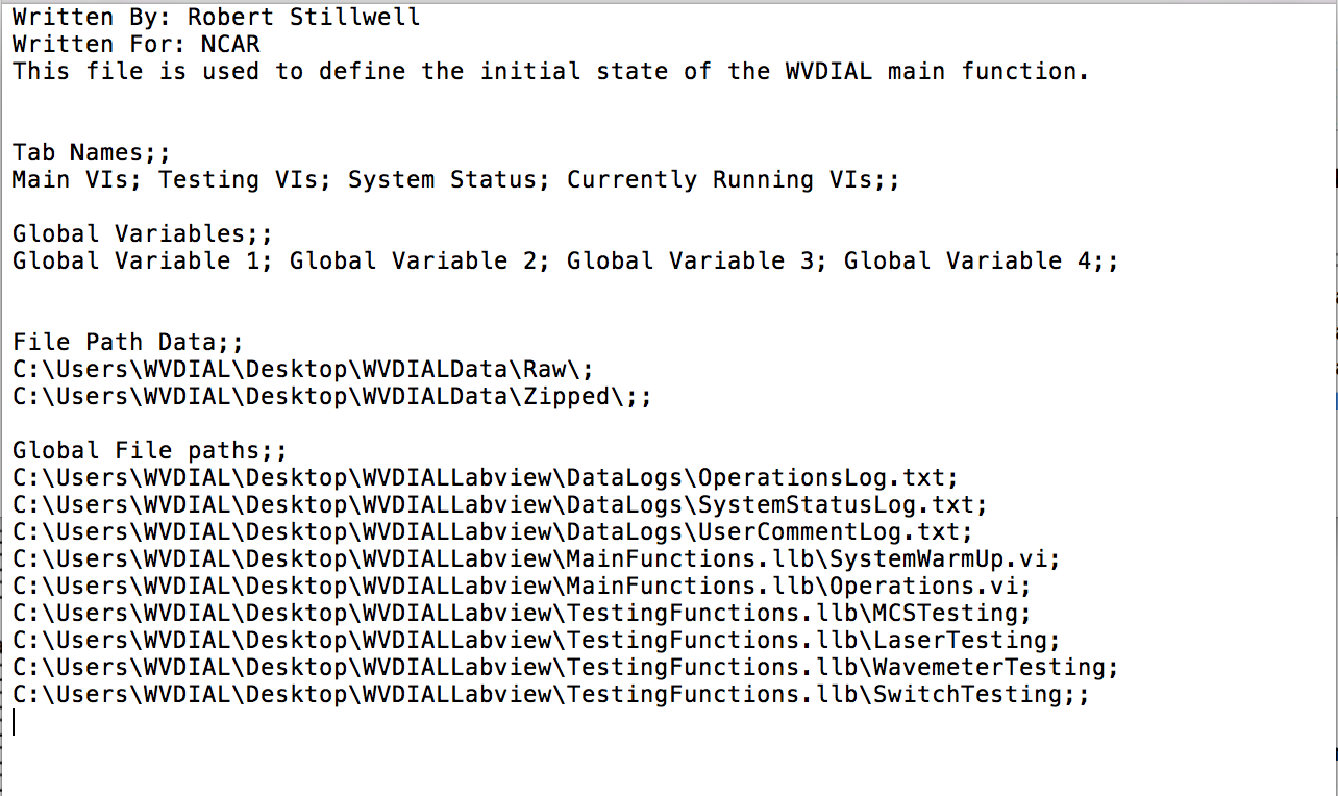
\includegraphics[height=3in]{Figures/ConfigureFileExample}
\caption{An example of the structure of a configure file. Variables are identified by a single name followed by two semi-colons. The next line has the required values delimitated by a single semi-colon with the end of line denoted by a double semi-colon.}\label{Fig:ConfigureFile}
\end{figure}

If a configure file has been edited and a revert to a default state is required, local changes to the configure file can be discarded and replaced with the defaults from the github repository. This is accomplished from the git bash terminal by navigating to the ConfigureFiles directory for the unit and running a command like - 

git checkout $ \langle $ConfigureFileToCheckoutFromGithub$ \rangle $  

If you want to replace the configure file in the github repo with a currently functioning configure file, then run these commands from the git bash after navigating to the ConfigureFiles directory for the unit - 

git add $ \langle $ConfigureFileToAddToGithub$ \rangle $ 

git commit -m ``comment describing the commit''

git push

This assumes that your local repo is up to date with the remote repo. Much, much more can be learned through a google search about Git/Github including branches, releases, etc... than i will be able to describe here. 



\chapter{Getting Started}
\label{CH-GettingStarted}

Now that the config files are together we can get started. Open The vi WVDIAL\_Main.vi and start the main container. It should look like figure~\ref{Fig-StartupContainer}. All functionality of the container is within a tabular control. The first tab holds what you see now, and when an operation mode is selected the functionality associated with that mode will open up in tabs that were defined in the configure files associated with that mode. The main container also has some readout information near the bottom of the screen as well as three buttons for permissions, comments, and an abort. For relampago deployment the permissions and comments are not hooked up to anything, but the abort button is hooked up and will stop the labview program. When you want to stop labview operations make sure to stop the current running mode (usually main operations) wait for it to fully stop (all the tabs will go away and the buttons on the main tab will return) and then hit the abort button. Another feature that you will notice when entering an operational mode is a child responsivness display on the right hand side of the screen shown in figure~\ref{Fig-Responsive}. That display will show the children that are currently being used, and will confirm their responsivness to the main container. 

\begin{figure}[!ht]\centering

\includegraphics[height=3in]{Figures/QMark}
\caption{The main container on startup.}
\label{Fig-StartupContainer}
\end{figure}

\begin{figure}[!ht]\centering

\includegraphics[height=3in]{Figures/QMark}
\caption{The display showing children as responsive.}
\label{Fig-Responsive}
\end{figure}

\newpage 



\chapter{Functionality}
\label{CH-Functions}

These are the things you can do with the software, represented by buttons in the main container. The operational modes that are called by the buttons on the main panel are:

\begin{enumerate}
\item{Warm up sub-function that brings all hardware to operational status. This includes things like warming the lasers and warming the etalons, which needs to be done before high quality data can be taken.}
\item{Main operations sub-function that performs all the mission critical hardware communication during data collection. This is discussed further in Chapter~\ref{CH-Ops}}
\item{A template sub function which brings up an empty child with minimal functionality.}
\item{Switches sub-function which tests our ability to control the switches.}
\item{Temp. Scan sub-function which sweeps through temperatures to test the lasers.}
\item{Testing sub-functions for individusal controls to check operational status of hardware pieces such as the wavemeter (laser locking), the MCS operation, or the weather station.}
\end{enumerate}

\section{Individual Element Controls}
The proposed software update parses the main hardware control function into sub-functions. These sub-functions serve to control individual elements of the WVDIAL, serve as simplified routines to warm up elements of the WVDIAL, or are to test out specific functionality in isolation of the rest of the unit. 

\subsection{MCS}\label{Sec:MCSSubFunction}

A sub-function that brings up two children. One does the communications via UDP to read the MCS, while the other is a set of controls to change the state of the MCS. These two functions are open in different tabs to seperate functionality. The first has three tabs, one to monitor photon counting returns, one to monitor power, and one that holds other controls for the software. In the other controls there are clusters for inputing where each return is plugged into the MCS, as well as readouts for other MCS related communications. In the Photon Counting tab there are controls for Channel and a Channel multiplier. This is used to scale up the display of one channel for comparison to other channels. This multiplicative factor only affects the display. The Channel selection here corresponds to the data channel cluster in the third tab. The tab which contains the MCSControls itself has four tabs, as the NCAR MCS has many settings. They are broken up by functionality as photon counting, power monitoring, other controls, and status readouts. 

\subsection{Weather Station}\label{Sec:WSSubFunction}

A sub-function that brings up the weather station child to monitor surface level temperature, pressure, relative humidity, and absolute humidity. There are controls here for update period and the com channel for the device. 

\subsection{Laser Locking}\label{Sec:LLSubFunction}

A sub-function that brings up the laser locking routines that controls laser wavelengths and the etalons. It has four tabs, one for controls, one for readouts, one for readouts of the data saving routines, and one for display of data collected. 

\subsection{Housekeeping}\label{Sec:HousekeepingSubFunction}

A sub-function that brings up one child whose responsibility is to relay information about the temperature of the container. Thermocouples are placed within the container in various positions which can be specified for writing into the data in the Configure\_WVDIALPythonNetCDFHeader.txt. This is primarily to help ensure that the climate control for the unit is functioning properly. There are controls for update period, the number of thermocouples attached to the unit, and for the ethernet communications information. 

\subsection{UPS}\label{Sec:UPSSubFunction}

A sub-function that calls the UPS child to monitor the state of the UPS Battery and power to the unit. The UPS child has a subroutine to automatically send out an email when the UPS Battery gets too low. There are controls for update period, how low the battery is allowed to get before shutting down or sending a warning email, and for the ethernet communications information. 

\subsection{HSRL Oven}\label{Sec:HSRLOvenSubFunction}

A sub-function that warms up the HSRL. This is not currently built, but the button on the front panel is there for the addition of the feature in the future. 

\subsection{Wavemeter}\label{Sec:WavemeterSubFunction}

A sub-function that brings up the wavemeter to read the wavelengths of the lasers. There are controls for update period, and for the ethernet communications information. 

\subsection{Thor 8000}\label{Sec:T8000SubFunction}

A sub-function that controls the Thor 8000 laser diode current control module. 

\subsection{Quantum Composer}\label{Sec:QCSubFunction}

A sub-function that controls the Quantum Composer timing unit. For the Relampago release the only functionality is to write, there is no read function. When writing to the QC you may have to click through a couple error pop ups in order to sucessfully set the state of the QC. As long as the Setting State light at the bottom of the display, then the state of the quantum composer was set. The controls for System Parameters and Channel Parameters are not set via config file, and this functionality is more advanced, so set the Quantum Composer with care. 

\subsection{Power Switches}\label{Sec:PowSwitchSubFunction}

A sub-function that controls the power switches.

\subsection{NetCDF}\label{Sec:NetCDFSubFunction}

A sub-function that brings up the NetCDF writer for reprocessing of data files. There are two controls, one for how many hours to back process data (minimum of three) and an update period which is how often you want the system to process data. Make sure that the hours to back process is greater than the update period so you don't miss processing of data. The larger the number of hours to back process is then the longer the processing with take to run. As a conservitive estimate you can run 24 hours of data in less than 10 minutes. 

\newpage 



\chapter{MainOps}
\label{CH-Ops}

This is the most fundamental part of the software. While deployed in the field this is the mode that the software will be running in for a large majority of the campaign. To begin main operations click the MainOps button. It will take a moment for all children to start but when they do you should see all children as responsive on the right hand side. The tab names are configurable via the Configure\_WVDIALMainOps.txt configure file. I will refer to them by their default names. 

The first tab is always Main Controls, which holds the controls to begin modes of operation. The next two are Raw Data and MCS Controls which are used to communicate with the MCS and gather photon counting and power data. The Laser Locking tab controls the wavemeter and is used to control the lasers and etalons. The UPS monitors the state of power to the unit and the UPS battery. The Adv. Visualization tab is used to display composite variables, but does not write any data. This tab could completely crash and would not affect the final data products in any way. The NetCDF tab is used to control the python scripts that write out the final and intermediate data products. Lastly the Weather Station tab controls the weather station. 

When you start main operations be sure that all children are reporting as responsive to the main container, then flip through the tabs to be sure each is responding as you would expect. For the Raw Data tab make sure that photon returns look reasonable, that peaks are showing up where clouds are present, that the data is changing on the expected interval (1/2 Hz by default), etc.... Go into the Laser Locking tab and make sure the wavemeter is responsive. There is a known problem with the wavemeter that causes it to return a default value instead of actual wavelengths, so make sure to give this 5-15 seconds for the wavemeter to respond with real values. If the unit is running not on the battery then check that the UPS is reporting a full battery, and if it is not then make sure the battery is charging and report the UPS behaviour. Check the Weather Station tab to ensure that the weather station is responsive with physically sensable values, the default frequency for weather station returns is 1/10 Hz so don't be suprised if it looks like it isn't updating. Lastly the NetCDF tab will begin by running the python on startup. This python code can take a minute to run so if the output and error boxes are empty then check that the PythonRunning light is lit. When the python is done running the output and error fields should be filled. If the python runs sucessfully the end of the output box should end with a Goodnight World line that has a time stamp. The error field is not empty even in the event of sucess. Seeing output in this field is not a problem or a bug, it should look like a series of paths to output files. If there is any error reporting in this field that is not a path to an output file, then that is an error, and needs attention. Attempts were made to log errors and warnings and the location of those error and warning files is printed at the top of the output. 

The data should be written to the Data directory, as well as being RSynced to an external hard drive connected to the unit, and lastly it should be RSynced to Eldora. Make sure that the data product is actually being written to each of these locations. 

If you've looked at all these tabs and checked the data output then congratulations, you're done. You can walk away and let the DIAL unit run for as long as needed. You can collect your final data products as described in chapter~\ref{CH-Data}.




\chapter{Data}
\label{CH-Data}

Data is saved in three locations, in the Data directory embedded within the software, on an external hard drive conneted to the DIAL unit, and on Eldora. The Data directory has several directories containing data in various stages. The final form of the data is the merged CFRadial files which is in the Data/CFRadialOutput directory, more on those below. Raw data is stored in two forms, NetCDFOutput which contains raw data in a NetCDF format, and in either binary or text format (child dependant) which is stored in seperate directories for each child. The merged CFRadial files should be the files you are interfacing with by default, but if for some reason those were not able to be written don't panic. As long as the binary and text files are being written then you have your data, and raw NetCDF files as well as the merged CFRadial files can be re-processed after the fact if nessicary. Raw NetCDF files are derived from the binary and text files, and merged CFRadial files are derived from the raw NetCDF files. 

\section{Merged Data Output}
\label{Sec-DATAOutput}

Merged files can be checked with a quick print script which is located in tempShare. That function is NetCDFQuickPrint.py. It can be called from the command line as - 

python NetCDFQuickPrint.py <pathToMergedFile>MergedFiles130000.nc WVOffline

Once you get the path to the merged file correct you can pick a data product that you want to plot. The options are (if they are present in the file) [WVOnline, WVOffline, HSRLCombined, HSRLMolecular, O2Online, O2Offline]. For Relampago there is no HSRL or O2 lasers so those selections are expected to error out if you are using this quick print script. Before it errors out it should show you the variables and dimentions so you can get an idea of what is in the file. The option of what to plot is currently limited to a photon counting selection, but hopefully this example script allows you to start reading the merged CFRadial files in python. 

When attempting to read these files in with Matlab, be sure to use the hdf5read functionality instead of the ncread functionality. This is a consequence of having chosen NetCDF4 as the format of the files and Matlab's interaction with NetCDF4's chosen string formatting. This is a known bug that has been submitted to Matlab, it is unknown when it will be addressed. Example Matlab code to read in these files is on Eldora. 


%%%%%%%%%%%%%%%%%%%%%%%%%%% Ending document %%%%%%%%%%%%%%%%%%%%%%%%%%%%
\end{document}
